\subsubsection{Functional Principle} \label{section:license-google-functional}
Google's approach is a network service which allows to query the trusted Google Play license server in order to determine whether the user has a valid license.
The library is provided by Google and the exact functionality can be studied by the developer since it is delivered in source code.\cite{munteanLicense}
\newline
It has to be manually integrated into the application by the developer and allows a simple checking with Google and has a callback for the reply.
The developer can decide when and how often the application should check its license.
Upon initiation, the library connects to the Google Play Service which manages the connection between the device and the license server.
It sends a request for a license check on the server to determine the validity of the license, whether the application was bought by the user.
This is similar to \gls{drm}.
Adding the library to the application does not alter the function of the application, it just addes a call.
While the library takes care of the complicated process, like the networking and webservice, and returns the response of Google Play as soon as it arrives, the developer only has handle the callback.
The developer is in full control what should happen with the response and whether access should be granted.
Figure~\ref{fig:lvl} gives an overview how the parts are connecnted. \cite{digipomLvl} \cite{developersLicensingOverview}
\newline
\begin{figure}[h]
    \centering
    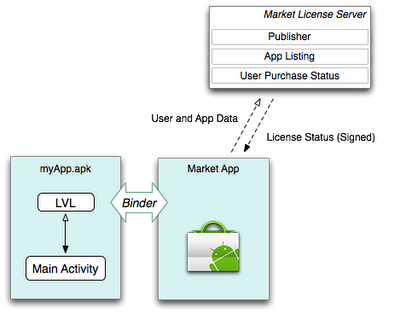
\includegraphics[width=0.8\textwidth]{data/lvl.png}
    \caption{Google's implementation of license checking \cite{developersLicensingOverview}}
    \label{fig:lvl}
\end{figure}
In order to start the validation process with the Google Server und to determine the license status of the application, additional information has to be provided.
The user has to initiate the call with  the package name of the application, a salt which has to be included in every call to ensure no attack has happened as well as the callback for asynchronous handling.
The Google Play Service then adds the primary Google account the application is executed with, the IMSI of the device
On the server Google checks whether the user has purchased the application and sends the corresponding response to the Google Play Service which passes it to the application. \cite{developersLicensingOverview}
\newline
The security of the response is very important.
It is achieved by public/private key encryption.
Each published application in the Play Store has a pair of keys of which the developer has to integrate the public key, which is visible to him, into the application in order to decrypt the communication which is encrypted by the server with the private key.
This way it the origin of the response is ensured as well as tampering detected.
\cite{munteanLicense}\cite{developersLicensingOverview}
\newline
This results in some restrictions for the application to run.
First of all, access to the internet is necessary as well since a connection to the Google Server has to be established.
In case this is not possible, an internal error will be triggered which results in the license not being verified.
Second of all, the Google Play Service has to be installed.
It comes preinstalled with the Google Apps which includes the Google Play store.
On the one hand, this is a prerequisite to legally aquire an application with the \gls{lvl}.
On the other hand, in case applications, with \gls{lvl} implemented, cannot bind to the Google Play Service and thus cannot verify the license status.
When the server is finally reached and the license is verified, it can be stored on the device and used in future requests in case no internet connection is available.\cite{developersLicensingAdding }\cite{developersLicensingOverview}
\newline
In summary this means the Google Play Service as well as a one time internet connection have to be present on the first startup in order to make the license check and, in case of the right answer, run the application.
It replaces the old copy protection, which is no longer supported, with a secure mechanism to control access to the application.
This license verification model can be enforced on all devices which have access to Google Play. \cite{developersLicensingAdding} \cite{developersLicensingOverview}
